\documentclass[10pt, letterpaper]{article}
\usepackage[spanish]{babel}
\usepackage[]{graphicx}
\usepackage[utf8]{inputenc}


\title{Moogle}
\author{Salma Fonseca Curbelo}

\begin{document}
    
    \maketitle

\begin{abstract}
    El siguiente documento describe los pasos que se siguieron 
    para desarrollar el primer proyecto de programación, 
    cuyo objetivo es  implementar el motor de búsqueda de Moogle!,
    una aplicación cuyo propósito es buscar inteligentemente un texto en un 
    conjunto de documentos.
\end{abstract}


    \newpage
        
        Al inicializar el programa, se ejecuta el método \textit{GetDocuments}, que se encuentra en la 
        clase \textit{Documents}. Este método primeramente obtiene la dirección de todos los archivos de
        textos en la carpeta \textit{Content}, para lo que se crea el string \textit{filepath} que se le asigna la 
        dirección de la carpeta a la que entrará y luego con la función \textit{GetFiles}, de la clase
        \textit{Directory} se obtienen las direcciones de todos los documentos de ella y se guardan en
        un array de string llamado \textit{docs}.

        \begin{figure}[h]

            \centering
            \label{imag: obtdocs}
            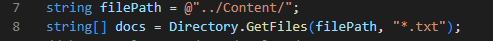
\includegraphics[width=11cm]{ObtenerDocs.png}
            \caption[]{\footnotesize Obtener direccion de documentos}

        \end{figure}

        Luego se lleva a cabo un ciclo foreach, que para cada dirección que se encuentra en \textit{docs},
        con la función \textit{ReadAllText} de la clase \textit{File}, se obtiene el texto de los documentos, 
        ignorando las mayúsculas con el método \textit{ToLower} y se guardará en una variable de tipo string 
        llamada \textit{document}. Después se crea una lista de string con cada palabra del texto,
        para separarlas se utiliza el método \textit{Split} de la clase \textit{Regex}, que cada vez que haya un 
        carácter que sea distinto a una letra (puede tener o no tilde) o un número, hace una división,
        devolviendo al final un arreglo de string con cada palabra del texto, el cual se convierte a
        lista con el método \textit{ToList}.

        Una vez creada la lista se creará un nuevo vector, que se le pasará como parámetro la lista 
        con cada palabra del texto y la dirección.
        
        \begin{figure}[h]
            \centering
            \label{imag:cargardocs}
            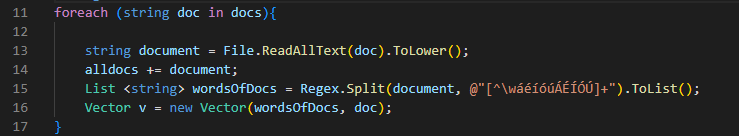
\includegraphics[width=10cm]{CargarDocs.png}
            \caption[]{\footnotesize Obtener contenido de documentos}
        \end{figure}

        La construcción del vector se lleva a cabo en la clase \textit{Vector}, que tiene como propiedad un
        string \textit{path} que será la dirección del texto, un entero \textit{cantidadPalabras} que representará la
        cantidad de palabras que tiene el vector, una lista de string \textit{vectorwords} con todas las 
        palabras y un diccionario \textit{TFIDF} de cada palabra con su valor de TF. Para construir cada
        vector:

        \begin{itemize}
            \item  a Vectorwords se le asigna la lista de string que recibe como parámetro.
            \item  a path se le asigna el string que recibe como parámetro.
            \item  a cantidadPalabras se le asigna el tamaño de la lista que se recibe,
             lo cual se determina con la función Count.
        \end{itemize}


        \newpage

        Cada vector que se cree se le añadirá a la lista de vectores \textit{files} de la clase \textit{Matrix}.

        \begin{figure}[h]

            \centering
            \label{imag: docvectores}
            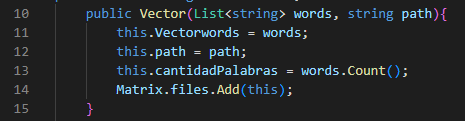
\includegraphics[width=10cm]{DocVectors.png}
            \caption[]{ \footnotesize Lista de documentos}

        \end{figure}

        Una vez terminado todo esto, a cada documento le corresponderá un vector.

Luego el método \textit{GetDocuments} entrará en otro ciclo que, para cada vector de la lista \textit{files} en la clase \textit{Matrix}, 
se llama al método \textit{CalculateTFIDF} y enviará como parámetro el vector. Este método se encuentra en la clase \textit{Matrix},
la cual tiene como propiedad la lista de vectores \textit{files} y un diccionario idf con todas las palabras y su valor
de idf.

\textit{CalculateTFIDF} comienza un ciclo foreach que por cada palabra del vector, si el diccionario \textit{TFIDF}
no la contiene, entonces se añadirá y se le asigna el valor 1, en caso de sí existir entonces se le aumenta uno al
valor de palabra.

\begin{figure}[h]

    \centering
    \label{imag: calculoTFIDF}
    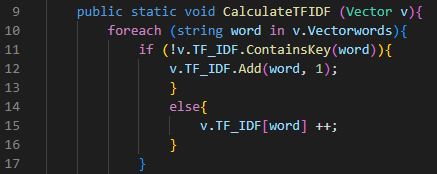
\includegraphics[width=9cm]{CalcularTFIDF.png}
    \caption[]{ \footnotesize Método para calcular repetición de palabras}

\end{figure}

Al culminarlo entra en otro foreach que recorrerá cada palabra que se encuentra en las claves del diccionario,
si esta no se encuentra en las claves del diccionario \textit{idf}, entonces añadirá y se le asigna el valor 1, en caso 
de sí existir entonces se le aumenta uno al valor de palabra.

\newpage

Y posteriormente se realiza el cálculo del TF de esa palabra, que sería la cantidad de veces que se repite la 
palabra en el documento (el valor que tiene asignado en el diccionario \textit{TFIDF}), divido entre la cantidad
de palabras del documento que es una propiedad del vector.

\begin{figure}[h]

    \centering
    \label{imag: TF}
    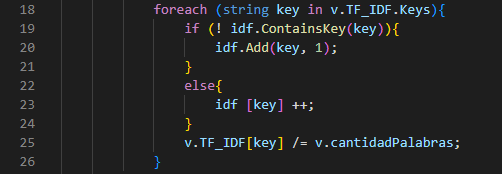
\includegraphics[width=9cm]{TF.png}
    \caption[]{ \footnotesize Método para calcular TF}

\end{figure}

Al haber hecho esto con todos los vectores se tendrá calculado el TF de cada palabra por documento y también se 
tendrá en cuantos documentos existe cada palabra.

El método \textit{GetDocuments} entre en otro ciclo foreach que para cada palabra clave del diccionario \textit{idf}, realizará 
el cálculo del IDF, que sería el logaritmo de la cantidad de documentos de la base de datos, que se obtiene con
la cantidad de vectores que contiene la lista \textit{file}, utilizando la función \textit{Count}, dividido entre la cantidad de
documentos que contienen la palabra (es el valor que tiene en el diccionario idf)

\begin{figure}[h]

    \centering
    \label{imag: IDF}
    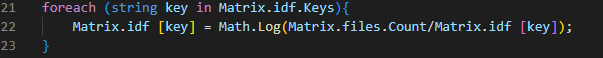
\includegraphics[width=13cm]{IDF.png}
    \caption[]{ \footnotesize Método para calcular IDF}

\end{figure}

Al finalizar todo esto se abrirá el programa con todos los documentos cargados, y los TF e IDF calculados.

Al usuario introducir lo que desea buscar, se ejecuta la función \textit{Search} dentro de la clase \textit{Moogle},
que recibirá como parámetro el query que se introdujo. Comienza convirtiendo dicho query a una lista de string \textit{query}, con el
método \textit{Split} igual que se utilizó anteriormente y llevándolo a una lista con la función \textit{ToList}. También se 
crea una lista de \textit{SearchItem}.

Comienza un ciclo que, por cada vector de la lista de vectores \textit{files}, crea una variable tipo double llamada 
\textit{score} que se le asigna el valor 0 para empezar. Entre en otro ciclo que para cada palabra de la lista \textit{query}, 
si esta se encuentra en las claves del diccionario \textit{TFIDF} y su valor en el diccionario \textit{idf} es mayor que 0.5 
(si fuera menor significa que la palabra se encuentra en la mayoría de los documentos por tanto no tendría 
importancia), se multiplica el valor del TF por el del IDF lo cual se le asigna a la variable double tfidf.

\newpage

Luego se realiza la siguiente operación:

\begin{equation}
    \centering
  \sum  tfidf \cdot  idf \cdot tf
\end{equation}
\\
Refiriéndoe al tfidf de la palabra en el documento, al idf propio de la palabra y al tf de la palabra en el query. Para saber la cantidad de veces que se encuentra la palabra en el query se
utiliza la función \textit{Count}.

\begin{figure}[h]

    \centering
    \label{imag: score}
    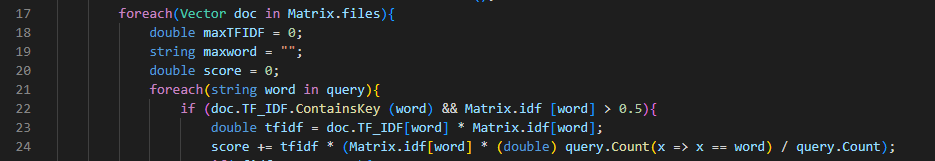
\includegraphics[width=9cm]{Score.png}
    \caption[]{ \footnotesize Método para calcular score}

\end{figure}

Al terminar esto con todas las palabras del query, si el score es mayor que 0, se le añade a la lista de 
SearchItem, llamada \textit{result}, el nombre del documento, que se obtiene a través de la función \textit{GetName},
el Snnipet, que se obtiene mediante la función \textit{Snippet} y el score.

Habiendo hecho esto con todos los vectores, se ordenan de manera descendente teniendo en cuenta el score y 
se convierta la lista a un array. Lo cual retorna la función y así se puede dar el resultado de la busqueda.

\begin{figure}[h]

    \centering
    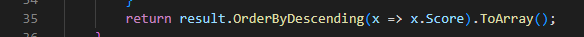
\includegraphics[width=13cm]{Scoredes.png}
    \caption[]{}

\end{figure}

La función \textit{Snippet}, de la misma clase \textit{Moogle} recibe un string con la dirección del documento, utilizando la
función \textit{ReadAllText} como se hizo anteriormente se obtiene el texto del documento y se crea un substring:

Si el tamaño del string recibido es menor de 150 caracteres entonces se devuelve todo el string con la función
Substring en 0; en caso de ser mayor entonces se hace el substring de los primeros 150 caracteres, 
igualmente con la función substring desde 0 hasta 149.

\begin{figure}[h!]

    \centering
    \label{imag: snippet}
    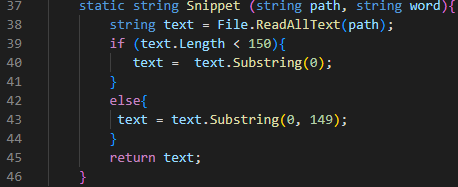
\includegraphics[width=9cm]{Snippet.png}
    \caption[]{ \footnotesize Método para crear el Snippet}

\end{figure}

 \newpage

La función \textit{GetName} con la dirección del documento, crea un substring que va desde el último '/ '
(con la función \textit{IndexOfLast} + 1) hasta donde empieza el txt, que se resta el \textit{IndexOf} de donde está txt 
menos el \textit{IdexOfLast} de '/' menos 1. IndexOf devuelve la posición del caracter u string que se pasa como 
parámetro. 
\\
\begin{figure}[h!]

    \centering
    \label{imag: docname}
    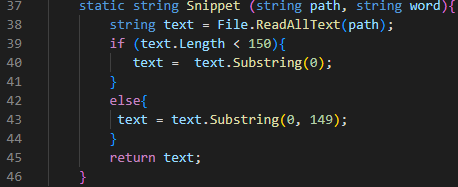
\includegraphics[width=9cm]{Snippet.png}
    \caption[]{ \footnotesize Método para obtener el nombre de documento}

\end{figure}

\end{document}